\chapter{Evaluation}
    In this chapter \acs{PATH} is tested and evaluated. For testing, programs with varying complexity are used; starting from simple programs ranging to more complex programs. 
    There are three main \nameref{sec:researchque}, which will be put to the test in Sections \ref{sec:ffa}, \ref{sec:ins} and \ref{sec:scalex}; validating \acs{PATH}.
    
    \section{Experimental Results}
    \par Programs from an increasing range of complexity were tested in this section. Individual opcode features of \acs{PATH} were verified with the simple functions found in \textit{project/tests/opcode}, logical functionality of \acs{PATH} (such as \acs{CFG} generation) was tested with 
    functions found in \textit{project/tests/logic}, and finally, general purpose testing was conducted via open source programs\footnote{obtained from \url{https://github.com/OmkarPathak/Python-Programs/tree/master/Programs}}. All functions passed the \nameref{sec:factgen}, \nameref{sec:cfimp} and \nameref{sec:irgen}
    stages, reporting satisfactory results. Performance results covering all functions can be found in Figure \ref{fig:resultsPATH}. 
    
    \begin{figure}
        \centering
        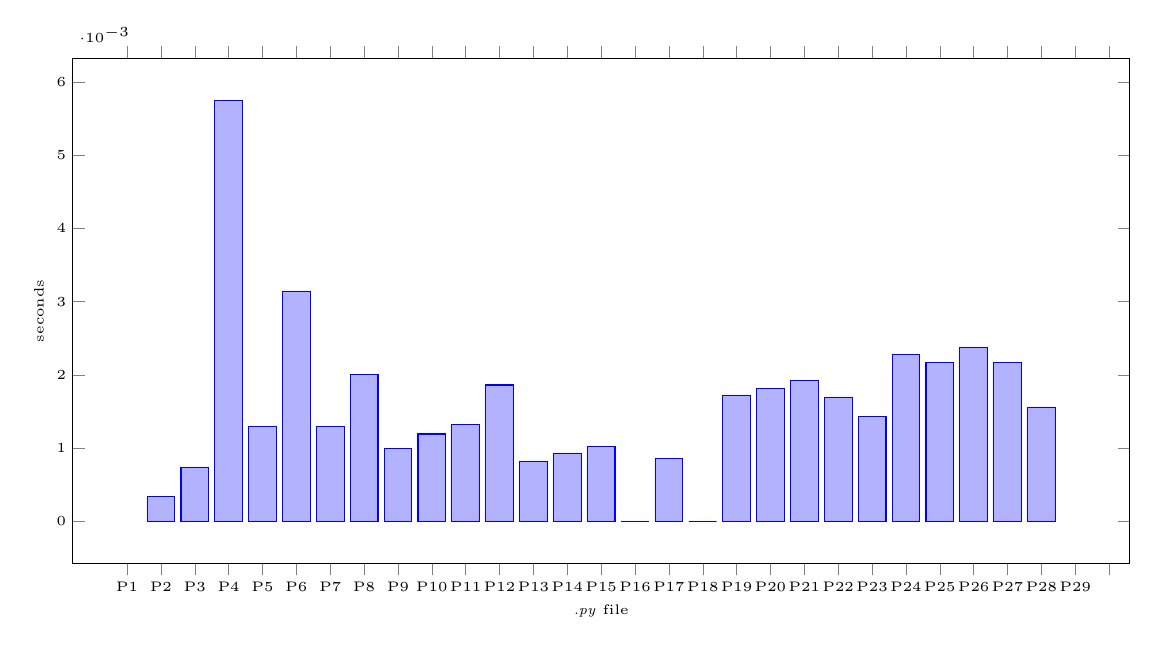
\begin{tikzpicture}
            \tiny
            \begin{axis} [ybar,height=8cm,width=15cm,xlabel={\textit{.py} file},ylabel=seconds,
                xtick={0,...,30}, xticklabels={P1,P2,P3,P4,P5,P6,P7,P8,P9,P10,P11,P12,P13,P14,P15,P16,P17,P18,P19,P20,P21,P22,P23,P24,P25,P26,P27,P28,P29}
                ]
                
                \addplot coordinates {
                    (1,0.0003352165222167969) 
                    (2,0.0007417201995849609) 
                    (3,0.005750894546508789) 
                    (4,0.0012981891632080078)
                    (5,0.003136873245239258)
                    (6,0.0013020038604736328)
                    (7,0.002003908157348633)
                    (8,0.0009911060333251953)
                    (9,0.001194000244140625)
                    (10,0.0013189315795898438)
                    (11,0.0018641948699951172)
                    (12,0.0008230209350585938)
                    (13,0.0009243488311767578)
                    (14,0.0010180473327636719)
                    (15,0)
                    (16,0.0008580684661865234)
                    (17,0)
                    (18,0.0017158985137939453)
                    (19,0.001811981201171875)
                    (20,0.0019237995147705078)
                    (21,0.0016949176788330078)
                    (22,0.0014328956604003906)
                    (23,0.002279996871948242)
                    (24,0.002176046371459961)
                    (25,0.0023789405822753906)
                    (26,0.002176046371459961)
                    (27,0.0015537738800048828)
                    
                };
                \end{axis}
        \end{tikzpicture}
        \normalsize
        \caption{Performance Metrics of \acs{PATH}}
        \label{fig:resultsPATH}
    \end{figure}

    \section{Research Questions}
    \label{sec:researchque}
        The research questions below aid in systematically investigating the need and use of \acs{PATH}. These questions are delved into more depth in Sections \ref{sec:ffa}, \ref{sec:ins}, and \ref{sec:scalex}.
        \subsection{How further analyses is facilitated}
        \par \acs{PATH} creates \textit{.facts} files. Such files contain metrics pertaining to the function analysed that are of interest to end users.
        These files' contents are tabulated in \nameref{table:facts_table}.
        \subsection{CPython invariants, and findings}
        \par Throughout this project, several undocumented findings have been concluded from results generated by \acs{PATH} processing the functions in \textit{project/tests}.
        The primary undocumented findings are listed below:
        \begin{itemize}
            \item Elementary Blocks in CPython do not retain any content on their frame stacks.
            \item \lstinline|LOAD_GLOBAL| is reserved for storing function names.
            \item Bytecode operations on the frame stack. 
        \end{itemize}
        These findings amongst others are further discussed in Section \ref{sec:ins}.
        \subsection{Scalability of \acs{PATH}}
        For \acs{PATH} to be of any practical use, it must be able to scale appropriately, and traverse through different function calls.  
        This is possible as it follows a recursive methodology when dealing with \lstinline|MAKE_FUNCTION| calls. \acs{PATH} 
    \section{Facilitating further analyses}
    \label{sec:ffa}
    \par Program analysis is a computationally intensive and time-consuming process. This process is facilitated by the use of automated tools, such as \acs{PATH}. The \textit{facts} generated 
    by \acs{PATH} are thought out in such a way so as to analyse functions and to enable any further analyses one might conduct. A prime example would be the potential to carry out a Data Flow Analysis with the 
    information generated by \acs{PATH}. For a Data Flow Analysis one requires a \acs{CFG} (generated as mentioned in Section \ref{sec:cfimp}), and data-flow equations for every node of the \acs{CFG}.
    A popular approach to Data Flow Analysis is the Reaching Definitions Method (See section \ref{subsec:dfa}). This would be facilitated with \acs{PATH} via the \acs{CFG} generated and the following \textit{.facts} files:
    \textit{StatementUsesLocal.facts} and \textit{PushValue.facts} (refer to \nameref{table:facts_table}); demonstrating that it does indeed reduce the engineering complexity of further possible analysis. 
    \par This tool enables teams to focus on the analysis itself, negating the need of the preliminary step for the creation of different intermediary representations to conduct analysis on. The fact that 
    there are not many professionals in this area makes complex analysis tools expensive and rare to come across.
        \subsection{Relating \acs{PATH} with current frameworks}
            \par In reality, program analysis cannot be simply bisected into two categories; it is more accurately depicted by the spectrum shown in 

            \begin{figure}
                \centering
                \begin{tikzpicture}
                    
                    \node[align=center] (staticstring) at(-6,0){Static\\Analysis};
                    \node[align=center] (Dynamicstring) at(6,0){Dynamic\\Analysis};
                    \node[align=center] (autostring) at(0,5){Automated Analysis};
                    \node[align=center] (manual) at(0,-5){Manual Analysis};

                    %%axis
                    \draw[very thick,latex-latex] (-4.4, 0) -- (4.4, 0);
                    \draw[very thick,latex-latex] (0, -4.4) -- (0, 4.4);
                    
                    %%background
                    \draw[ultra thin, gray, step=.5cm] (-4.3,-4.3) grid (4.3,4.3);

                    \tkzDefPoint(-3.9,0){static}
                    \tkzDefPoint(0,4){symEx}
                    \tkzDefPoint(-3.6,-4){manual}
                    \tkzDefPoint(3.4,2){dynamic}
                    \tkzDefPoint(3.6,-4){debug}
                    \tkzDrawPoints[color=black,shape=circle,fill=black!70,size=8](static,symEx,manual,dynamic,debug);
                    
                    \tiny
                    \node[] (text1)[right=of static] at (-5,0.25) {Static Analysis};
                    \node[] (text2)[right=of static] at (-0.5,3.8) {Symbolic Execution};
                    \node[] (text3)[below=of static] at (-3.1,-2.45) {Manual Auditing};
                    \node[] (text4)[below=of debug] at (4,-2.45) {Debugging};
                    \node[] (text4)[above=of dynamic] at (4,1.1) {Fuzzing};

                    \normalsize

                \end{tikzpicture}
                \caption{Spectrum of Program Analysis}
                \label{fig:spectrumPA}
            \end{figure}
            \subsubsection*{Similar Frameworks}
            \par \acs{PATH} is a pure basic program analysis framework, in which its stereobate lies with the generation of an \acs{IR}. This framework takes inspiration from several other
            Static frameworks which operate similarly:
            \begin{description}
                \item[doop]A Java pointer and Taint Analysis framework that conducts analysis by the Soufflé Datalog Engine \cite[]{bravenboer2009strictly}.
                \item[soot]A Java optimization framework, providing analyses ranging from \acs{CFG} construction to Taint analysis \cite[]{vallee2010soot}.
                \item[Gigahorse]An Ethereum analysis framework, specializing in the decompilation of smart contracts \cite[]{grech2019gigahorse}.
                \item[Vandal]A fast and robust security analysis framework for Ethereum smart contracts \cite[]{brent2018vandal}.
            \end{description}
            \par The frameworks mentioned above are {\bfseries pure} program analysis frameworks, whereby the analysis is conducted on an \acs{IR}. 
            
            \subsubsection*{Different Frameworks}


    \section{Insights}
    \label{sec:ins}
    \par 
    \section{Scalability Experiments}
    \label{sec:scalex}
    \section{Case Study}